\documentclass{acm_proc_article-sp}

\usepackage{makeidx}  % allows for indexgeneration
\usepackage{listings}
\usepackage{amsmath}
\usepackage{graphicx}
\usepackage{subfigure}
\usepackage{color}
\usepackage[allowmove]{url}

\definecolor{lightgray}{rgb}{.9,.9,.9}
\definecolor{darkgray}{rgb}{.4,.4,.4}
\definecolor{purple}{rgb}{0.65, 0.12, 0.82}

\lstdefinelanguage{JavaScript}{
  keywords={typeof, new, true, false, catch, function, return, null, catch, switch, var, if, in, while, do, else, case, break},
  keywordstyle=\color{blue}\bfseries,
  ndkeywords={class, export, boolean, throw, implements, import, this},
  ndkeywordstyle=\color{darkgray}\bfseries,
  identifierstyle=\color{black},
  sensitive=false,
  comment=[l]{//},
  morecomment=[s]{/*}{*/},
  commentstyle=\color{purple}\ttfamily,
  stringstyle=\color{red}\ttfamily,
  morestring=[b]',
  morestring=[b]''
}

\lstset{
   language=JavaScript,
   backgroundcolor=\color{lightgray},
   extendedchars=true,
   basicstyle=\footnotesize\ttfamily,
   showstringspaces=false,
   showspaces=false,
   numbers=left,
   numberstyle=\footnotesize,
   numbersep=9pt,
   tabsize=2,
   breaklines=true,
   showtabs=false,
   captionpos=b
}

\newcommand{\FIXME}[1]{{\color{red}\textbf{FIXME: #1}}}
\newcommand{\javaCode}[1]{\texttt{#1}}

\title{A Mulitplayer Augmented Reality Game for Android Phones
\numberofauthors{2}
\author{
\alignauthor Ben Lickly \\
       \affaddr{University of California, Berkeley}\\
       \affaddr{Berkeley, CA, USA} \\
       \email{blickly@eecs.berkeley.edu}
\alignauthor Darren Kuo \\
       \affaddr{University of California, Berkeley}\\
       \affaddr{Berkeley, CA, USA} \\
       \email{darrenkuo@eecs.berkeley.edu}
}
}


\begin{document}
\maketitle

\begin{abstract}
Here we present an augmented reality game for the Android smartphone platform
that is an homage to Namco's Pacman, but played in the real world.  The game is
controlled by running around the real world, which is captured by the phone's
GPS sensor. These readings are uploaded to a server running on Google
Appengine, which takes care to coordinate and mediate the actions of each of
the individual players.  In order to test the efficiency of the infrastructure,
we have constructed a phone simulator in Go that can simulate many phones
simultaneously while running on a standard desktop computer. Using this
simulator, we have simulated games that have up to 256 fake phones. At this
scale, the main bottlenecks in the system are the time it takes to display all
of the players on the screen of the Android phone, and the latency of the
server to handle all of the concurrent writes.
\end{abstract}

\section{Introduction}
Augmented reality refers to a view of the physical world that has been
augmented with additional computer-generated information, creating a
sort of hybrid between virtual reality and the real world. Existing
applications include games, sightseeing guides, navigation aids, and
automatic translators.

Recent years have seen the success of a new class of video games with
new methods of input, such as Dance Dance Revolution, Nintendo Wii,
Playstation Move, and Microsoft Kinect. We see Augmented Reality games
where players leave their game machine and physically move around the
real world as a logical extension of this progression

\section{Related Work}
There already exist a handful of augmented reality games for android. Probably
the most similar to the game presented here is ``Zombie, Run!"~\cite{ZombieRun},
in which the player plays as a human that must run away from an indeterminate number of zombie enemies. One of the largest differences in the games is
that the enemies in ``Zombie, Run!" can move in any direction, including
through walls, whereas in our game we have specifically defined a map in
such a way that players and enemies move on the same grid of streets.

Other types of smartphone augmented reality games also exist, such
as those for ghost hunting~\cite{SpecTrek}, navigating mazes~\cite{ARLabyrinth},
and augmented reality role playing games~\cite{ParallelKingdom}.


\section{Gameplay}
The game presented here is an untraditional game on the Android platform.
Rather than using the touchscreen or keys as input to control the gameplay,
we make use the GPS sensor on the phone to allow players to control their character.

The game is an homage to Namco's Pacman, in which a player tries to eat all
of the dots in a maze without getting eaten by enemy ghosts. In the original
game, the player is controlled by a joystick and the maps are fixed, whereas
in our augmented reality version, the player is controlled by moving around,
and the map is dependent on the layout of the real-life streets in the
neighborhood in which the game is being played.


In our game, the user can creating a map of his/her neighborhood with
the included map editor.
This defines which area of their real life neighborhood are in bounds during
the course of the game, and where the other players, enemies, and ghosts are
created.
The map editor also allows users to save customized maps to a server,
so that the maps can be persistantly backed up, and also so that players
can share maps with each other.

In order to start playing, a user simply selects the desired map to start a new game. The player is then presented with a map of their real world location populated with dots that must be run over to be ``eaten". Unlike traditional pacman, our game is multiplayer, allowing multiple players to play in a single game.
After starting a new game, the user can invite his/her friends to join the
game.

Each player must pick a role in the game, either a pacman or a ghost. The
goal of the pacman character is to eat all the food dots on the map, and
a score count is kept of how many dots each pacman player has eaten.
The ghost players, on the other hand, aim to eliminate all the pacman players.
Just like the original pacman game this game requires strategy to plan out a
path to eat dots, but also to anticipate the movement of other real human
players.

\section{System Architecture}

\begin{figure}
\centering
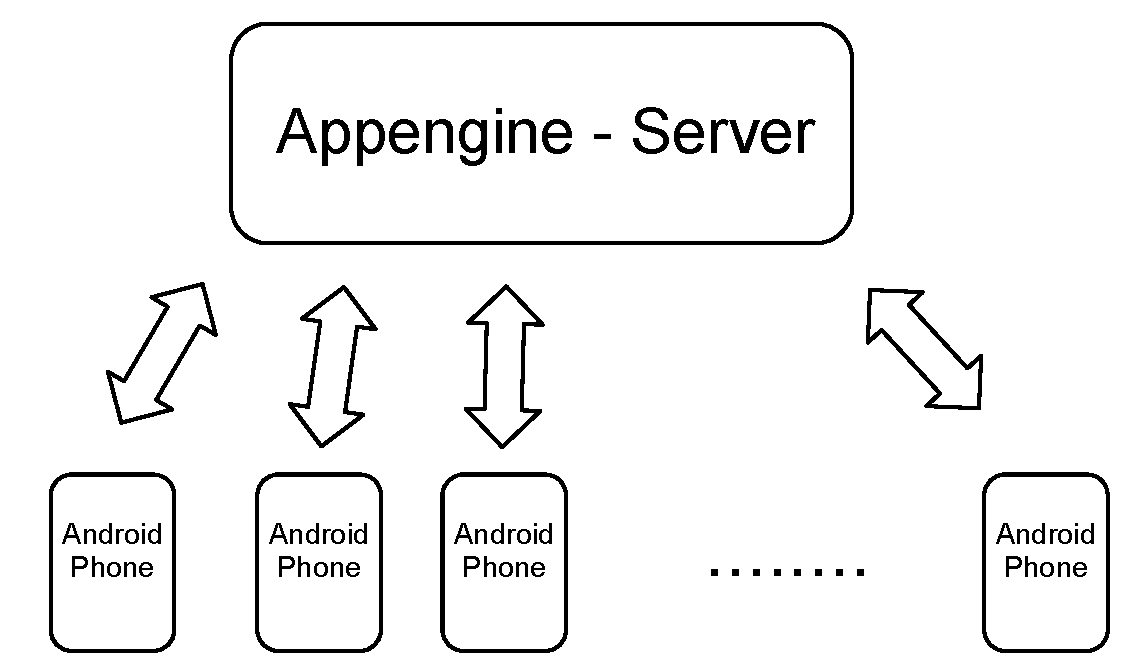
\includegraphics[scale=0.4]{figs/ServerArchitecture}
\caption{A server on Google Appenigine is used to coordinate communication between the phone clients.}
\label{fig:ServerArchitecture}
\end{figure}

Our augmented reality Pacman game is built in a client/server architecture as
shown in Figure~\ref{fig:ServerArchitecture}, where the server runs on Google's
Appengine service, and the clients are smartphones running the Android 2.2
operating system.  The server has an API that can be accessed through HTTP
connections, and the clients use this API in order to maintain a consistent
view of the world when playing a multiplayer game.

In practice, there are three methods used for sending data from the server to
an application running on an Android device:
\begin{itemize}
\item Phone-initiated polling of the server for data.
\item Interception of specifically crafted SMS messages.
\item Android Cloud to Device Messaging
\end{itemize}

Polling is the simplest approach, where the phone simply queries the server at
a given interval. The disadvantages depend on the polling rate. At low polling
rates, polling suffers from high latency, and at high polling rates, it can
consume more power and shorten battery life compared to other techniques.

Receiving information from the server through SMS is a much lower power
solution. In this approach, the app must register for the permission to read
incoming SMS messages, and then relies on the server to send messages from a
specific number with a given format. This approach has the disadvantage that it
requires unconventional permissions that may make users suspicious, and it is
difficult and expensive to deploy widely, especially when dealing with
international phone numbers. It is also unusable on devices like tablets that
may have 3G data coverage, but no phone number.

Android Cloud to Device Messaging (ACDM) is a service created by Google
specifically for push notifications, and is newest and most advanced approach.
ACDM uses Google infrastructure to allow communication of lightweight messages
of up to 1024 bytes. Servers communicate directly to Google servers, from which
the messages are relayed to Android phones through their Google user accounts.
The disadvantages of ACDM are that it is not available for versions of Android
prior to 2.2, and also that it can only send messages to phones that are logged
in to a Google user account.

Since the game mechanics require phones to contact the server regularly anyway
to update their locations, the overhead of the polling approach seemed most
reasonable. The ACDM could be another option that could potentially lower the
latency in some situations. The restriction of message size to 1024 bytes,
however, meant that updates in larger games would not always fit in a single
message, increasing complexity.


\subsection{Server}

We used a python webserver running on top of Google's Appengine
service. Google's Appengine service provides many advantage for our
Android app. The service has a built-in high replication datastore,
which implements the Paxos Algorithm~\cite{lamport01paxos} to
synchronize data across data centers in real time. The datastore
supports high availability for reads and writes, making it suitable
for our purposes.

The server is responsible for the following features:
\begin{enumerate}
\item Storing and retrieving of maps.
\item Creation of new games and querying of games in progress.
\item Support for joining games and generation of dots.
\item Keeping track of player locations.
\item Keeping track of which dots still exist.
\item Resolve when players are killed by enemies.
\end{enumerate}


\subsubsection{Map storage and retrieval}
Besides keeping track of information during gameplay, the server
is also responsible for storing maps and allowing players to retrieve
and use those maps. Here, we make use of the Appengine
datastore to store our maps using the \texttt{TextProperty}.
In an earlier iteration we tried to use the similar \texttt{StringProperty}
to store maps, but found problems. In particular, the
\texttt{StringProperty} can only store up to
500 characters and the value could be indexed for filtering and
ordering operations. For our usage, we only need to save and retrieve whole
maps, so the indexing feature is unnecessary. In addition, large maps
can easily grow above 500 characters, so the \texttt{TextProperty} field
was more appropriate.


\subsubsection{Creating and querying games}
The server also keeps track of which games are in progress. This is simpler
than the map storage and retrieval since creating a game does not involve
saving a large map representation. The work of generating of unique game
identifiers and querying of existing identifiers, however, is identical.

\subsubsection{Joining games and generating dots}
Like saving a map, joining a game requires the server to record information
about the player who has joined the game so that other players can all
see the player who has joined.

Additionally, the location of the dots on the map must be drawn by each
player's phone, so the initial location of the dots is returned to each player
after he or she joins the game.  Since the map format (shown in
Listing~\ref{lst:MapFormat}) does not include information about the location of
the dots, it must be generated by the server before players join the game. The
way that dots are generated is simply by spacing them out at a fixed distance
along all roads that are included in the game map.

\subsubsection{Tracking players}
Since the server is required to know where all the players are, it
must have some way to retrieve the most updated location of each
player and store it for other players to retrieve that
information. This protocol is designed to wait on the client. Despite
the existence of various technologies for servers to push data to
clients, we decide to go with the simple implementation of client
driven update.

When the client (player's phone) receives a GPS update, we will post
that location to the server to update our current position and
propagate our location to other players. As a response, the client
will receive a list of other player's locations. In this
implementation, we introduced wait time (queue time) for each
player's location on the server. There is this notion of how ``fresh''
the location data is, since the staleness of the location information
of each player, solely depends on how often the client decides to send
in their location.

\subsubsection{Eating dots}
Initially, we had the server resolve eating of dots. Now, we offset
that some of that responsibility to the client. The client will
specify which dot it wants to eat.
This allows for the client to quickly update its display that a point
has disappeared before getting a response from the server.
The server, then, needs to only resolve the race condition of who ate
the dot first in the case that two players simultaneously tried
to eat the dot. The format of this response is simply the number of
points that the client gained for its attempt.
If the client was attempting to eat
a dot that has already been eaten, then the server will return 0
points for the dot. If the client was the first player to request eating
a particular dot, then the server returns the full point value for eating
a single dot.

Another advantage of this implementation is that it means that
\url{/post_position} can be made more efficient, as it does not not need to
enumerate all the available dots when it responds to every request.  If
required, the delay caused by this calculation would increase the latency of
the request.

\subsubsection{Pacman being caught by the ghost}
This feature is also semi implemented on the client. The client will
send out a request when it detects the player captured a ghost (if the
player is a pacman). However, there are more steps to verify here than
eating dots. The server will check if the players are indeed close
together using the server location information about each player.

\subsection{Client}

The clients are implemented as native Android apps that run on any
Android platform of version 2.2. or higher.  Since we only had a limited
supply of physical phones for testing, we also implemented fake clients,
or ``phone simulators" that behave similarly to the Android devices, but
can be simulated in large numbers from a single desktop computer. These
are discussed in more detail in Section~\ref{sec:phoneSimulators}

There are two overall responsibilities of the client: map editing,
and playing the game.

\subsubsection{Map Editor}
The Map editor allow users to create customized maps and save it to
the server. The map editor uses Google's direction API
\cite{GoogleDirection} to find routes between two points. This
functionality is used when a user draws a map in the map editor. The
map editor also allows users to link points and delete points (along
with any related edges).

%\begin{figure}
%\centering
%\includegraphics[scale=0.4]{figs/MapEditor}
%\caption{The Map Editor provide the users with a simple interface to create new maps for gameplay.}
%\label{fig:MapEditor}
%\end{figure}

\subsubsection{Game Mapview}
The Game Mapview is used for the main course of this app - the
Gameplay. 

When a player is starting a game, he/she request to join a game and
the server returns a list of food dots (described in
\ref{newgame}). The game mapview is responsible for displaying the
dots and removing dots when a user is close enough to some food dots.

During the game, the Game Mapview is charged with the task of updating
the server whenever the location of the player changes. The Game
Mapview listens on the GPS location. Whenever there is a GPS location
change, the client use the new location to update the
gameplay. Although this is not entirely true, the client doesn't
update the server with every single new GPS location, since this can
easily consume all the phone's resources and bandwidth. The client
actually waits $0.5$ seconds between updating locations. The Game
Mapview will get a response with all the other player's location and
display those players on the map.

The client's game loop for a Pacman can be described as follows:

\begin{enumerate}
\item If player's location is updated $0.5$ within of the last update, we do nothing.
\item Else, we update our location on the server and get other player's updated location.
\item We also check if our location is close enough to any food dots. If so, request to eat a food dot.
\end{enumerate}

The client's game loop for a ghost is even simpler and can be descrbied as:

\begin{enumerate}
\item If player's location is updated $0.5$ within of the last update, we do nothing.
\item Else, we update our location on the server and get other player's updated location.
\end{enumerate}

Since the interaction between a pacman and a ghost is resolved on the
server, the game loop for a client is even simpler. However, it might
be a better design decision to implement this interaction in a way
that is similar to dots eating to reduce the amount of processing done
on the server.

\subsection{Game Protocol/API}
To implement the system described above, we implemented the following API:

\subsubsection{\url{/save_map}}
This method is responsible for handling the storing of new maps. A
request to this method should contain the contents of the map. The
return value would be an unique ID for the map.

\emph{Arguments:} map content in json.\\
\emph{Response:} Unique ID associate with that map.

\medskip
\begin{lstlisting}[caption=Map format in json,label={lst:MapFormat}]
[{ 'id' : <int>,
   'user_added' : <bool>,
   'lat' : <int>,
   'lng' : <int>,
   'neighbors' : [<int>]}+]
}]
\end{lstlisting}

\subsubsection{\url{/get_maps}}
This method allow users to get a list of map ID to allow the users to
pick the map to start a new game with.

\emph{Arguments:} None required.\\
\emph{Response:} A list of map IDs in json format.

\subsubsection{\url{/get_map}}
This method is responsible for retrieving stored maps. A request to this
method should contain an ID for a map that has been previously saved. The
return value contains the map contents in the format described in
Listing~\ref{lst:MapFormat}.

\emph{Arguments:} Map ID associated of map to read. \\
\emph{Response:} Map content in json.


\subsubsection{\url{/new_game}}\label{newgame}
This method create new games on the server for players to join for a
game of pacman. We required a map ID to start the game.

\emph{Arguments:} Map ID to start the game.\\
\emph{Response:} The unique game ID associated with the game.

When a game is create on the server, food dots are generated for the
map. Each player that joins the game will receive a list of existing
dot in the map.

\subsubsection{\url{/get_games}}
This method returns a list of game IDs of all games in progress, useful
for querying before joining a game.

\emph{Arguments:} None required.\\
\emph{Response:} A list of game IDs in json format.

\subsubsection{\url{/join_game}}
A player may join a game by requesting this method with a game ID and
a location (defined as a latitude and longitude).

\emph{Arguments:} Game ID to identify which game to join.\\
\emph{Response:} Player ID for requesting player and a list of initial food dot locations in json.

The method returns an unique player ID, which is used by the player
when posting location updates. The server refers to all players solely by
their player IDs.

\subsubsection{\url{/post_position}}
Whenever a player's GPS location gets updated, we want to make sure
that the player's location on the server is also updated.

\emph{Arguments:} Player's ID, game ID and location.\\
\emph{Response:} All the other player's locations and whether the requesting player is alive or dead.

The method is responsible for updating the player's location on the
server and also returning the other player's location. Furthermore,
any elimination of players are resolved on the server. Therefore, the
response includes the status of the player (i.e. dead or alive).

\subsubsection{\url{/eat_dot}}
Instead of having the server do the calculation of which dots are
eaten by which players, the phone calculates this locally. The
clients will specify which dots the player is eating and the server
will resolve the concurrency part of the problem.

\emph{Arguments:} Game ID and dot ID.\\
\emph{Response:} Score that the player gained for eating the dot.

Note that there is nothing preventing the users from cheating by
requesting to eat all the dots at the beginning of the game. This
security/unfairness aspect of the game is further discussed in the
future work (Section~\ref{future}). We aim to build a fast system for
friendly players, not adversarial programmers.

\section{Measurements}
\subsection{Phone Simulators}
\label{sec:phoneSimulators}
In order to get a meaningful evaluation of the entire architecture, we
need to have more than just measurements of latency in the simple
two-phones case.  In order to get a clear picture of how well the
architecture will scale, we would like measurements of how well the
system handles increasing load.  The most natural way to measure load
in our system is by increasing the number of phones playing the game,
but acquiring that number of hardware phones only for testing was
infeasible.  Instead, we built a phone simulator that can be run on
the computer and simulate the interaction of any number of phones
interacting with the server. We still do the latency measurements from
the real phones, since we want to take into account the potential
differences in latency between 3G and Wifi connections, but phone
simulators allow us to vary the load on the server in a realistic
way. Since creating more players for the game also means that the real
phones need to display more players on the screen, this load test is
also a way of testing how efficiently the players are drawn on the
screen of the handheld devices.

\subsubsection{Simulator Architecture}
The phone simulator is written in Go~\cite{GoLang}, and can create an arbitrary
number of concurrent threads that each simulate a single phone.  Each
simulated phone first queries the server requesting to join a specific
game, and gets back it's player id.  It then uses that player id to
generate random movement around a fixed point at a given update rate
(in the examples here, we have used a 1 second update rate as that is
the update rate used by the real phones). The simulator also logs all
of the responses from the server and when all communications are sent
and received, which would allow computation of server latency.  Since
we are more interested in the server latencies for real phones,
however, we do not use the simulator latencies in the results in the
following section.

\subsection{Measuring Latency}\label{measuring}

There are many difficulties with trying to measure latency in a
distributed system.  The most naive solution would be to simply time
from when one GPS reading is calculated on one phone to when that
updated position is displayed on another. The problem with this, of
course, is time itself is not totally ordered in a distributed
system~\cite{Lamport:1978:TCO}.

\begin{figure}
\centering
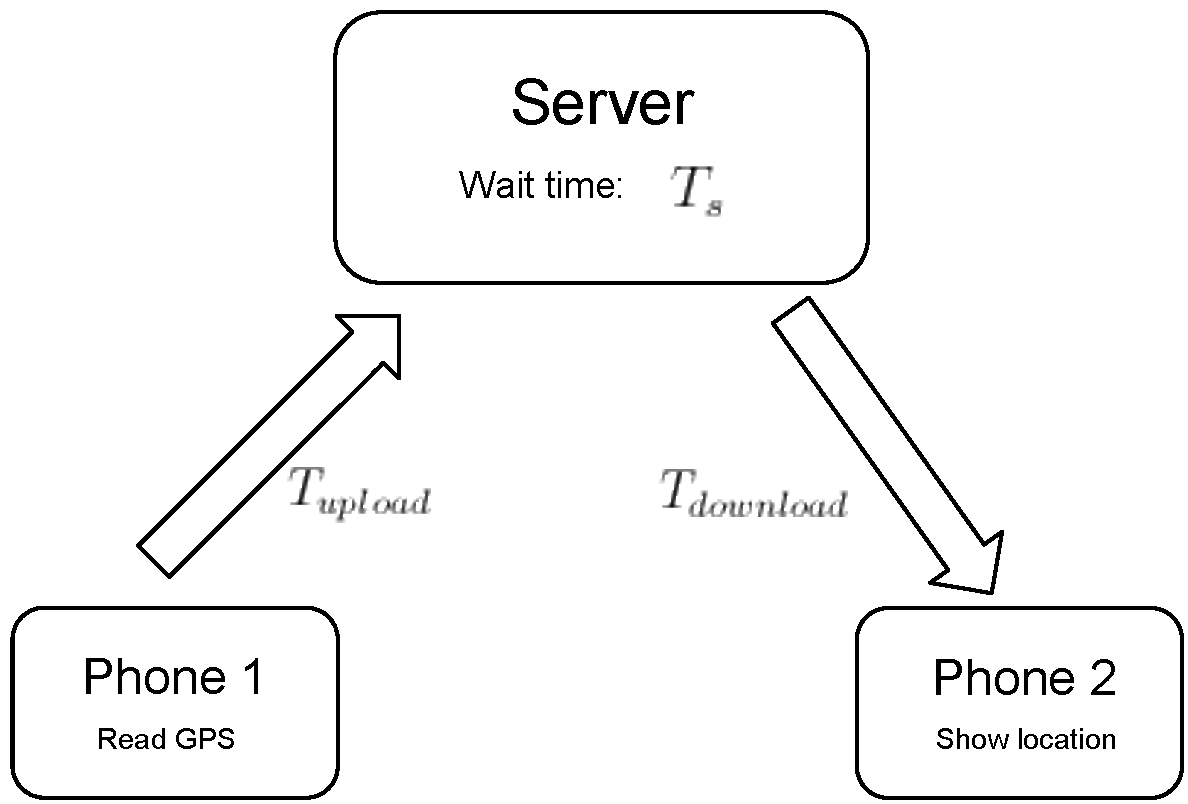
\includegraphics[scale=0.4]{figs/LatencyExplanation}
\caption{Latency can be broken down into three constituent pieces.}
\label{fig:LatencyExplanation}
\end{figure}

One solution would be to synchronize the notion of time on the phone.
If they could be synchronized within some known time bound, then we
could use timestamps and have a bound on the error of that
calculation.  Since phones include GPS and GPS includes a notion of
time, this is a feasible solution.

Another solution would be to measure a round trip time.  It is
important to make sure that the round trip time includes multiple
phones, since we are interested in the time that it takes to propagate
information from one phone to another.  One approach would be to time
the round trip time of the following set of events.  On a single phone
acquire a GPS reading, post it to the server, and then subsequently
request updates of other phones' positions from the server until they
change.  Under certain atomicity assumptions (namely that the reading
of positions and posting of GPS update is all done in an atomic and
isolated fashion) and network assumptions (that the network delivers
packets in order), getting an updated position from another phone
after posting your own update would be enough to guarantee that the
other phone had seen the original GPS reading.  Unfortunately, this
approach is complex and brittle, and many of the assumptions do not
necessarily hold in practice.

A third approach is one that combines observation on the phone with
observation on the server.  Rather than try to get an exact
measurement of any particular point-to-point or round-trip flow of
information, it merely tries to measure statistically certain subflows
that can be summed up to find a statistical measure of a likely
point-to-point flow.  The basic idea is that the latency for a GPS
reading to move from the GPS receiver on one phone to the screen on
another is made up of three parts:

\begin{enumerate}
\item the time that it takes to get from the GPS receiver on the first phone to the server ($\tau_{up}$),
\item the time that the reading waits on the server before it is queried by the second phone ($\tau_{s}$), and
\item the time that the reading takes to get from the server to the screen of the second phone ($\tau_{down}$).
\end{enumerate}

Since the second part is handled completely on the server, measuring
it is easier than the first and third part.  The key insight for
solving this problem is noticing that there is a certain degree of
symmetry among the phones, especially if we average over many
measurements.  It is likely that the latency for a reading to get from
the server to one phone will be very close to the latency to get from
the server to another.  Making this (reasonable) assumption allows us
to measure the sum of the first and third parts by simply measuring
the roundtrip time of two separate GPS measurements as seen by a
single phone.  That is, if we assume a certain degree of symmetry
among the phones, we can measure the time it takes to upload one GPS
measurement and then receive a different GPS measurement from the
server, and take that as a proxy for the sum of the first and third
measurements.  Summing this with the time measured on the server
between the GPS measurement being posted and being read by another
phone gives us a very accurate overall latency for reading-to-display
across multiple phones.

\begin{figure*}[pth]
\centering
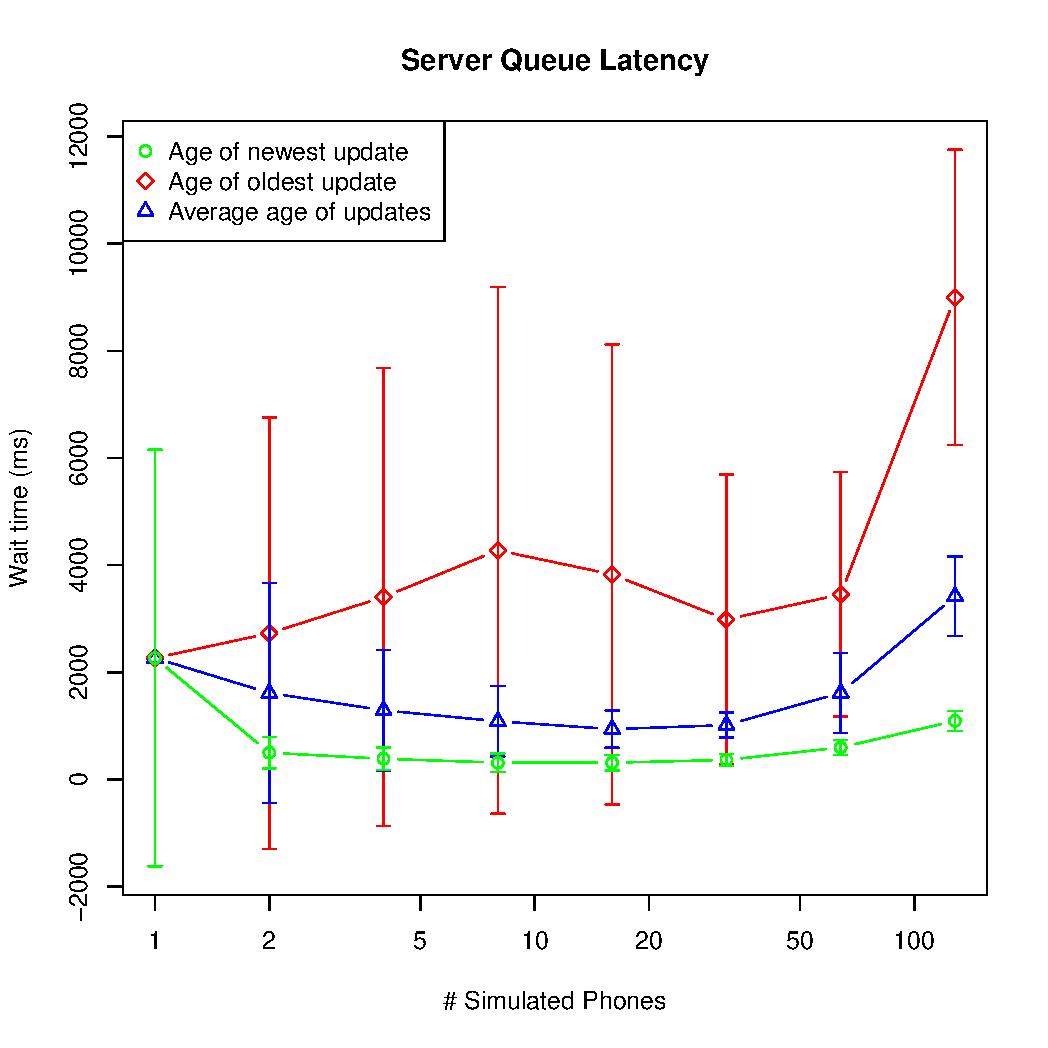
\includegraphics[scale=0.6]{figs/serverQueueLatency}
\caption{The highest, lowest, and average age of data fetched from the server.}
\label{fig:serverQueueLatency}
\end{figure*}

\begin{figure}[pb]
\centering
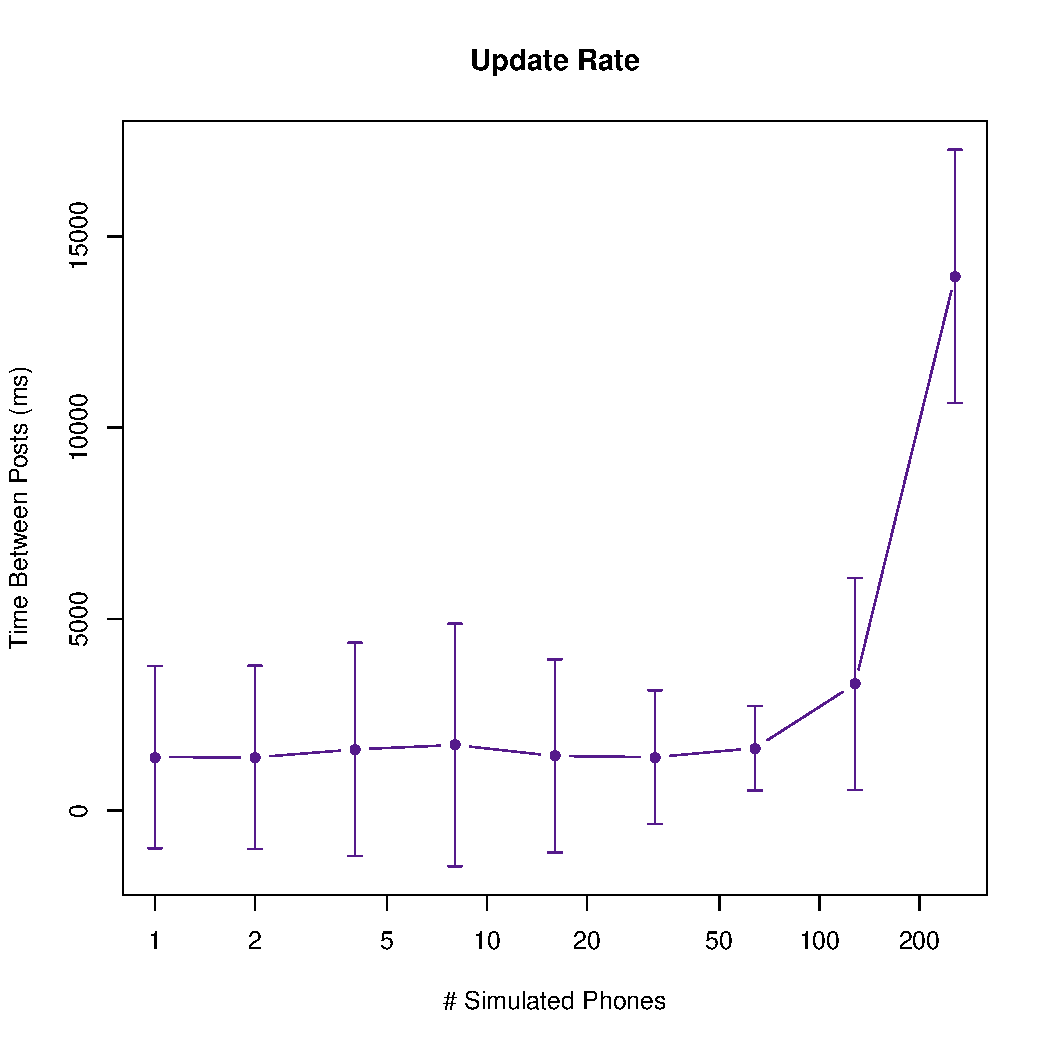
\includegraphics[scale=0.52]{figs/phoneUpdateRate}
\caption{The overall rate of post requests by the phone.}
\label{fig:phoneUpdateRate}
\end{figure}

\begin{figure}[pb]
\centering
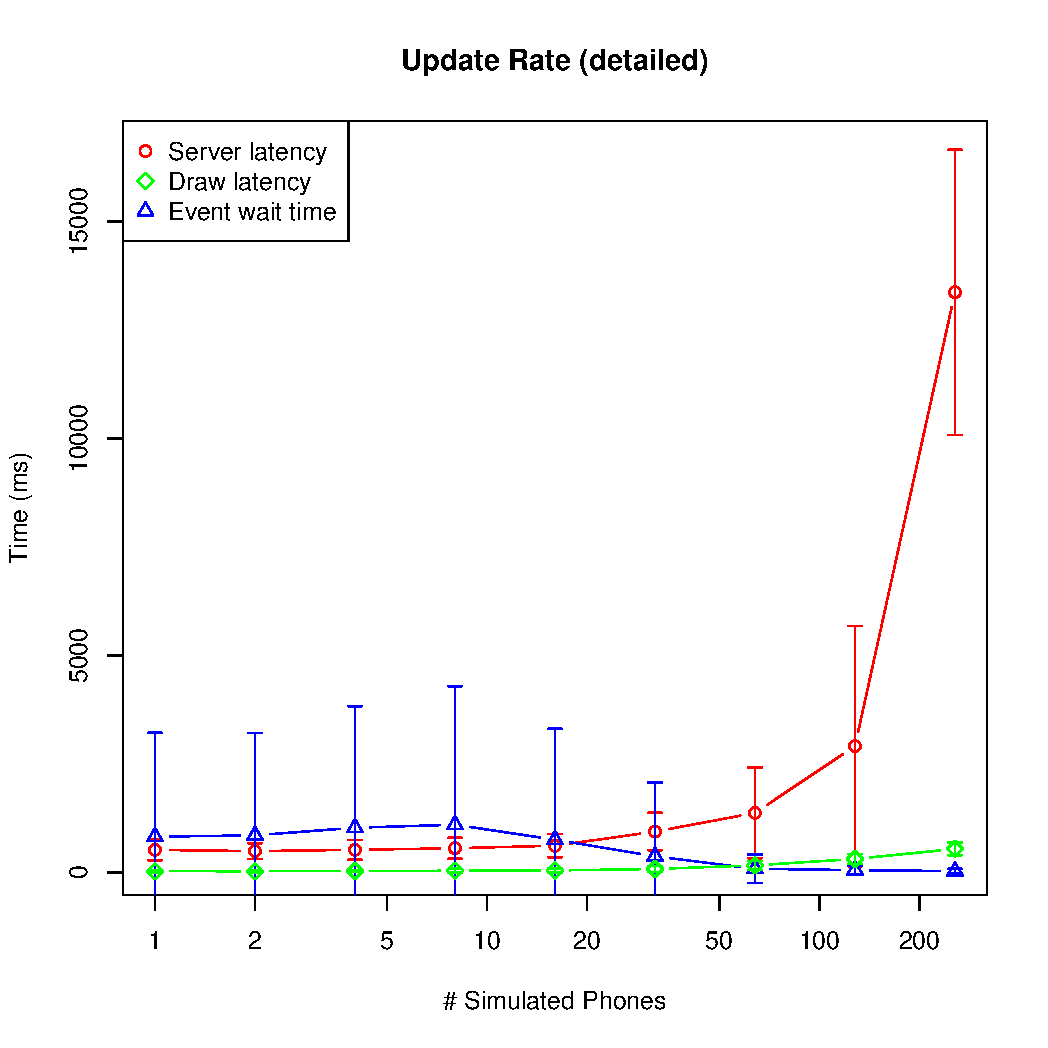
\includegraphics[scale=0.5]{figs/phoneUpdateRateDetailed}
\caption{The update rate can be broken down into server communication time, drawing time, and the wait time between GPS readings.}
\label{fig:phoneUpdateRateDetailed}
\end{figure}

\subsection{Results}
In order test how the system handles in response to high load, we ran
experiments in which we had one real phone play the game, and also included
a varying number of simulated phones running the phone simulators that
also interacted with the server using the same API as the real phone.
During 9 experiments each with a number of simulated phones ranging from 1
to 256, we measured data about latencies of various operations both on the
server and on the real phone.

\subsubsection{Server Queueing Latency}

In Figure~\ref{fig:serverQueueLatency}, we see the measure of the time that each GPS reading waits on the server before it gets read.  Since a single query of the \url{/post_position} method returns the GPS location of all other players, measuring the freshness of the data returned is not straightforward. If each of the GPS readings contained in the response to one request have been waiting on the server for different amounts of time, what is the most useful way to discuss the queue wait time for that request?
One way to measure this freshness would be to keep track of which GPS reading contained in the response was oldest, and report that as the queue time for the response. Another way would be to look at the newest GPS reading contained in the response. Yet another way would be to simply take the average queue wait time of all the readings contained in the response.
Figure~\ref{fig:serverQueueLatency} shows the average queue wait times by all three of these metrics as they vary with respect to server load.
Note that when there are only two phones (one real and one simulated), each request returns only a single GPS update, and all three metrics are identical.
It is interesting to note that the wait time of the newest update and average update actually decrease as phones are added up to 16 phones. This seems to be due to the fact that update requests are more likely to be spread evenly over time when there are a critical mass of phones making the requests.



\begin{figure}[t]
\centering
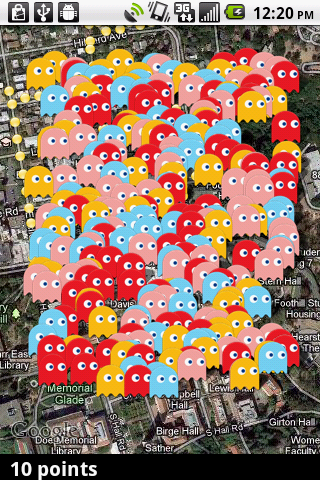
\includegraphics[scale=0.45]{screenshots/bigswarm}
\caption{The phone becomes less responsive when too many objects are drawn to the screen.}
\label{fig:256Ghosts}
\end{figure}

\subsubsection{Phone Update Rate}
The other source of latency is that of the time it takes to communicate between the phones and the server. These can conceptually be broken down into two independent parts, the time it takes to upload a reading to the server  ($\tau_{up}$), and the time it takes for a phone to download the reading ($\tau{down}$). Since both of these actions happen within a single API call (to \url{/post_position}), it is easier to measure the sum of these times than individually. To do so, we simply measure from the phone the overall latency of a single round trip of the \url{/post_position} API call.

\begin{figure}[t]
\centering
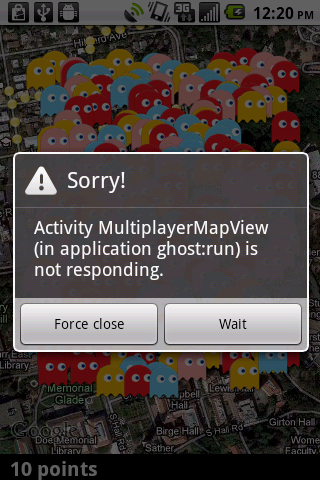
\includegraphics[scale=0.45]{screenshots/sorry}
\caption{When too many objects are drawn, the game can not be continued and must be quit.}
\label{fig:256GhostsSorry}
\end{figure}

Nominally, the phones try to make requests updating their positions every $0.5$ seconds, but in practice, the rate at which the phones are able to update depends on the load on the server and the latency of making the previous request. Figure~\ref{fig:phoneUpdateRate} shows how the overall request rate of the phone varies with respect to the number of simulated phones providing additional load.
Figure~\ref{fig:phoneUpdateRateDetailed} shows a breakdown of where this latency comes from. We originally suspected that the reason for increased latency with too many phones was a result of the drawing time for having too many objects on the screen. the latency from drawing so many objects on the screen was the driving force for increasing the time between updates on the phone, but Figure~\ref{fig:phoneUpdateRateDetailed} suggests that this is not the case.  Here we see that as the number of simulated phones increases past about 32, the latency of contacting the server becomes the dominant contributor to overall latency. One other interesting note involves the event wait time, or the time the phone spends idling between GPS updates.  When there is enough slack to have a relatively long idle period between finishing receiving one update and making the next GPS reading, not only is the event wait time high, as would be expected, but the variance is also high. Once the deadlines for making GPS readings start to be missed due to long server latencies, however, the even wait time disappears.
Because the phone slows down considerably with an increasing number of objects
are drawn to the screen, we initially assumed that the screen rendering time
was the bottleneck that caused a slow update rate for experiments with large
numbers of simulated phones. In a run with 256 simulated ghosts, such as that
shown in Figure~\ref{fig:256Ghosts}, the screen becomes completely unresponsive
and a dialog to close the app appears. Because the drawing is done in a
separate thread, however, it does not block the progress of the GPS updates to
the server, and our data shows instead that server latency is the primary cause
of slow update rates during games with very large numbers of players.

\subsubsection{Phone Signal Strength}
One more concern about having a multiplayer game was about the effect of the
signal strength of the phone on the latency of the communication with the
server. The concern was that as players ran through parts of the map that
may have had less strong cell signal, then the latency to the server may
increase. If this happened, then the game would be much less effective when
played in arbitrary locations that may have less strong cell coverage.

In order to test this hypothesis, we ran a series of experiments with a simple
one player game, moving the phone around to a variety of positions with
different signal strength, logging the latency of server queries and the
signal strength measurements available from the Android platform. Since the
phones used in this experiment were CDMA phones, the interfaces available
%
%   public int getCdmaDbm ()
% Get the CDMA RSSI value in dBm
%
%   public int getCdmaEcio ()
% Get the CDMA Ec/Io value in dB*10
%
to us were the \javaCode{getCdma()} and \javaCode{getCdmaEcio()} interfaces
of the \javaCode{android.telephony.SignalStrength}
provider~\cite{SignalStrengthAndroidDocs}.
The \javaCode{getCdma()} method returns the value of the received
signal strength indicator, which is a measure of the power of the received
signal is dBm.
The \javaCode{getCdmaEcio()} method returns a ratio of the pilot signal energy
to total received energy in units of dB, and is a measure of how clean the
received signal is.

\begin{figure}[t]
\centering
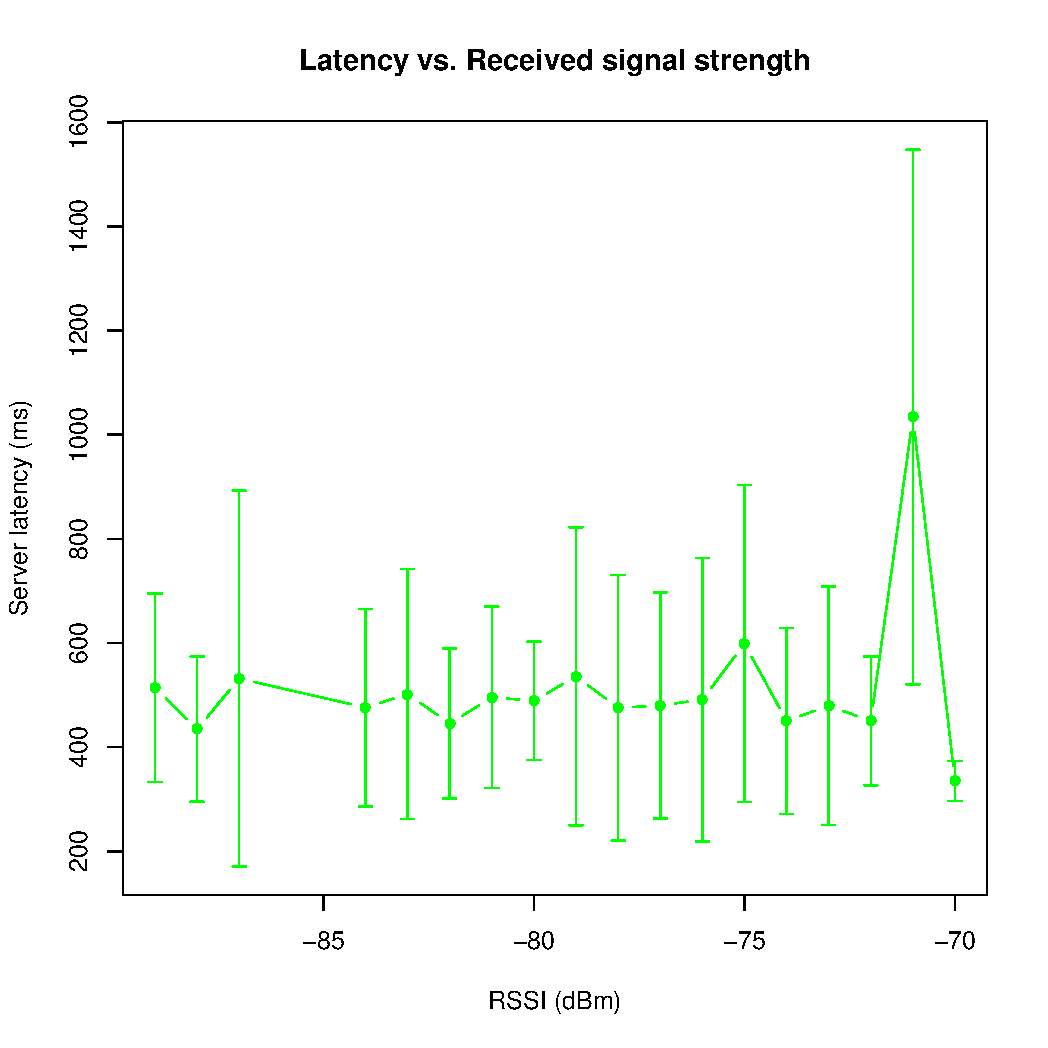
\includegraphics[scale=0.5]{figs/latencyVsRSSI}
\caption{Server latency as affected by received signal strength.}
\label{fig:latencyVsRSSI}
\end{figure}

\begin{figure}[t]
\centering
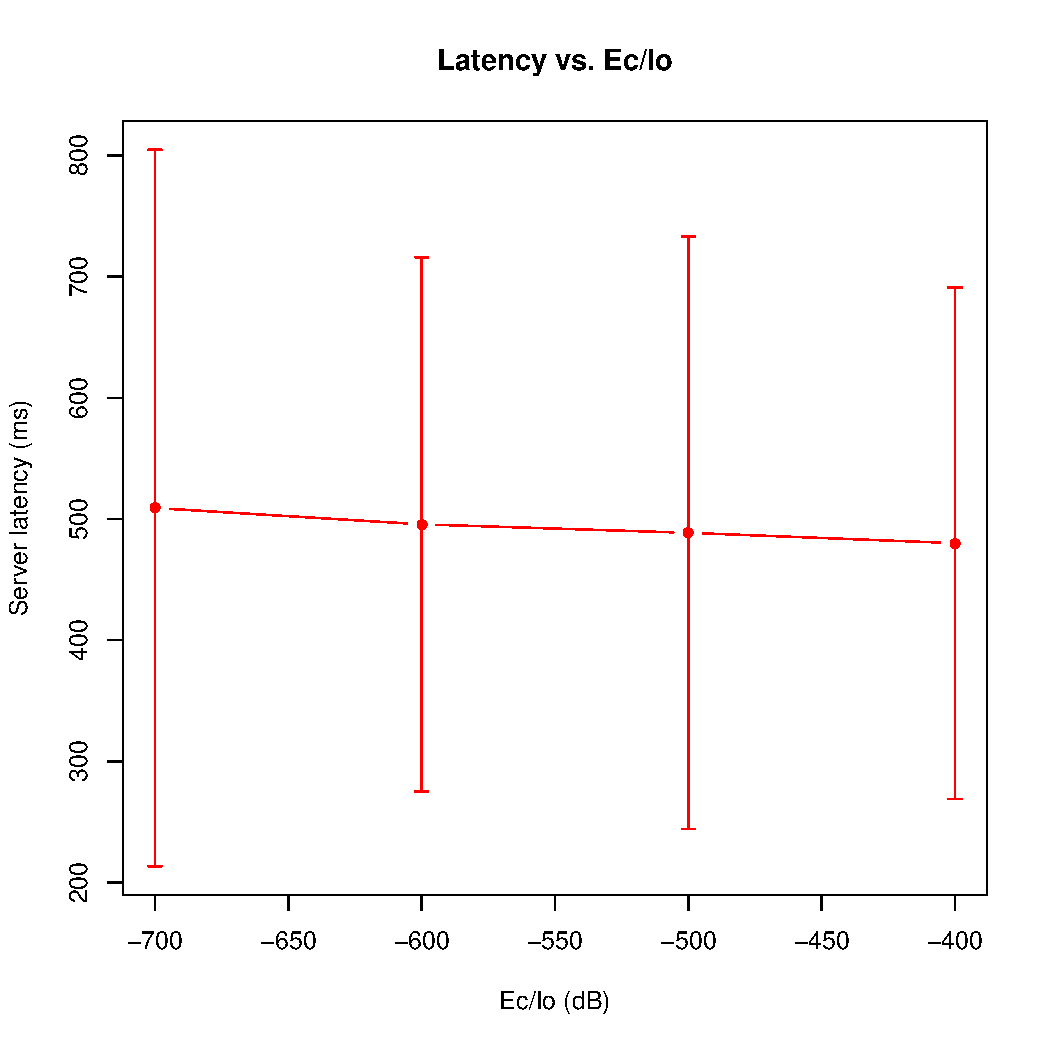
\includegraphics[scale=0.5]{figs/latencyVsEcIo}
\caption{Server latency as affected by pilot strength.}
\label{fig:latencyVsEcIo}
\end{figure}

There are many avenues for future work on this project.  The implementation
presented here did not take into the account of cheating that could take place
by unathorized clients or other abuse of the game API.  For example, a
malicious player could obtain all the dot information and request to eat all
the dots using a script. The lack of authentication makes it possible for
anyone who knows the location of the server to interfere with the gameplay.
Player could even potentially create their own Android app or modify the
existing one to make it send out fake GPS locations.  More work to make the
interaction between the server and the client more secure, such as including
user authentication, could make the game more fair.

The server latencies with respect to the received signal strength and pilot
signal are shown in Figure~\ref{fig:latencyVsRSSI} and
Figure~\ref{fig:latencyVsEcIo}, respectively. We were surprised to find that
there was no correlation between signal strength ans latency to query the
server. While it is clear that a phone with a sufficiently weak signal will be
unable to query the server at all, we found that for signal strengths within
the normal operating ranges that we were able to vary, signal strength had no
effect on latency. For other applications, it may be interesting to compare
signal strength with data bandwidth, but we did not try to make any such
comparison.

\section{Future work}
\label{future}


Currently, the player icons on the screen are moved only when updates are
received from the server.  When there is high latency, this creates a feeling
that the other players are performing ``teleportation'' due to thier ability to
cover a large distance instantaneously.  More work can be done to predict and
display the direction and speed of each player to make the animation of each
player's movement more smooth, without making the gameplay slower. With this
feature, the movement of players could appear less choppy without requiring
more frequent server updates.

Furthermore, the Android mapview is somewhat slow, since the overlay items (a
ghost or a pacman) includes other useful features (click listerns, dragging
support, etc), which are useless features for our purposes. A new
implementation that only support displaying of the icons could speed up the
system. Additionally, not all players and dots are on screen at all times
during gameplay.  We could potentially limit the map to only display set area
to allow for some optimization on map tile drawing and icon projections.

Certain data structures are better optimized for representing items in space, such as k-d trees~\cite{Bentley:1975:kdtrees}. These could potentially be used for storing the locations of the dots and players and to make the operations of checking when dots are eaten or players killed more efficient.

Another appengine feature that we would like to have used but did not have time
for was that of task queues~\cite{TaskQueuesAppengine}, which allow tasks that
are not responses to HTTP requests to be run on the server, effectively
giving a notion of independent threads.  The most obvious application of this
to our game would be to implement AI tasks for autonomously controlling
extra ghost or pacman characters in a way analogous to the phone-based client.
This would allow games with more players than human users on phones, and would
also allow for single player games that are still played over the server.


Aside from allowing the implementation of AI agents, task queues can be used
for managing other aspects of the server that are best handled asynchronously,
such as identifying games that have ended or were abandoned by the players.
Currently a game persists indefinitely, until the data is manually deleted from
the datastore on appengine, so a game deleting task queue could act as a
garbage collector for the server by and terminate games that have no players.


% FIXME: Do we need this stuff?
On the other note, we can also add more features to make the gameplay
experience more interesting. One of the idea could be the existence of
power pallets on the map. The pacmans will enter an invincible mode
for a short duration and would be able to eliminate ghosts from the
map. Other features could include a fog of war environment, an idea
taken from an undergraduate AI class, CS 188. During fog of war, the
player can only see other player that are within a certain
distance. The existence of food dots are also inaccurate. Pacman
player can see where the food dots are, but they won't be able to know
if the dots are still there until they are close enough.

Other even more exciting features can include a special featured
map. Equal number of players start on each side of the map. When a
player is on his/her own side, the player is a ghost and can eliminate
intruders. When a player is on the enemy's side of the map, the player
is a pacman and can eat dots. The team loses when it runs out of
dots. These variations of pacman games provide some defensive and less
deterministic gameplay experience.


\section{Conclusion}

We have here presented a rudimentary multiplayer augmented reality game for
Android phones. We have stress tested the whole system to find that the display
performance and server latency to be the primary constraints under very high
load conditions, but both are acceptable under normal loads.  We have presented
several possible directions for future development, including both new features
and ways to overcome the latency and display performance issues under high
load.  All of the development for this project, including the source code for
the Android app, the Appengine server, the phone simulator for stress testing,
and even this paper are publicly available, and can be accessed from
\url{https://github.com/blickly/ghostrun}.

\bibliographystyle{plain}
\bibliography{refs}
\end{document}
